
% Template for Elsevier CRC journal article
% version 1.0 dated 13 October 2009

% This file (c) 2009 Elsevier Ltd.  Modifications may be freely made,
% provided the edited file is saved under a different name

% This file contains modifications for Procedia Computer Science

%%%%%%%%%%%%%%%%%%%%%%%%%%%%%%%%%%%%%%%%%%%%%%%%%%%%%%%%%%%%%%%%%%%%%%%%%%

%% This template uses the elsarticle.cls document class and the extension package ecrc.sty
%% For full documentation on usage of elsarticle.cls, consult the documentation "elsdoc.pdf"
%% Further resources available at http://www.elsevier.com/latex

%%%%%%%%%%%%%%%%%%%%%%%%%%%%%%%%%%%%%%%%%%%%%%%%%%%%%%%%%%%%%%%%%%%%%%%%%%

%% The '1p' and 'times' class options of elsarticle are used for Elsevier CRC
\documentclass[1p,times]{elsarticle}

%% The `ecrc' package must be called to make the CRC functionality available
\usepackage{ecrc}

%% The ecrc package defines commands needed for running heads and logos.
%% For running heads, you can set the journal name, the volume, the starting page and the authors

%% set the volume if you know. Otherwise `00'
\volume{00}

%% set the starting page if not 1
\firstpage{1}

%% Give the name of the journal
\journalname{Procedia Computer Science}

%% Give the author list to appear in the running head
%% Example \runauth{C.V. Radhakrishnan et al.}
\runauth{}

%% The choice of journal logo is determined by the \jid and \jnltitlelogo commands.
%% A user-supplied logo with the name <\jid>logo.pdf will be inserted if present.
%% e.g. if \jid{yspmi} the system will look for a file yspmilogo.pdf
%% Otherwise the content of \jnltitlelogo will be set between horizontal lines as a default logo

%% Give the abbreviation of the Journal.
\jid{procs}

%% Give a short journal name for the dummy logo (if needed)
\jnltitlelogo{Procedia Computer Science}

%% Hereafter the template follows `elsarticle'.
%% For more details see the existing template files elsarticle-template-harv.tex and elsarticle-template-num.tex.

%% Elsevier CRC generally uses a numbered reference style
%% For this, the conventions of elsarticle-template-num.tex should be followed (included below)
%% If using BibTeX, use the style file elsarticle-num.bst

%% End of ecrc-specific commands
%%%%%%%%%%%%%%%%%%%%%%%%%%%%%%%%%%%%%%%%%%%%%%%%%%%%%%%%%%%%%%%%%%%%%%%%%%

%% The amssymb package provides various useful mathematical symbols
\usepackage{amssymb}
%% The amsthm package provides extended theorem environments
%% \usepackage{amsthm}

%% The lineno packages adds line numbers. Start line numbering with
%% \begin{linenumbers}, end it with \end{linenumbers}. Or switch it on
%% for the whole article with \linenumbers after \end{frontmatter}.
%% \usepackage{lineno}

%% natbib.sty is loaded by default. However, natbib options can be
%% provided with \biboptions{...} command. Following options are
%% valid:

%%   round  -  round parentheses are used (default)
%%   square -  square brackets are used   [option]
%%   curly  -  curly braces are used      {option}
%%   angle  -  angle brackets are used    <option>
%%   semicolon  -  multiple citations separated by semi-colon
%%   colon  - same as semicolon, an earlier confusion
%%   comma  -  separated by comma
%%   numbers-  selects numerical citations
%%   super  -  numerical citations as superscripts
%%   sort   -  sorts multiple citations according to order in ref. list
%%   sort&compress   -  like sort, but also compresses numerical citations
%%   compress - compresses without sorting
%%
%% \biboptions{comma,round}

% \biboptions{}

% if you have landscape tables
\usepackage[figuresright]{rotating}

% put your own definitions here:
%   \newcommand{\cZ}{\cal{Z}}
%   \newtheorem{def}{Definition}[section]
%   ...

% add words to TeX's hyphenation exception list
%\hyphenation{author another created financial paper re-commend-ed Post-Script}

% declarations for front matter

\begin{document}

\begin{frontmatter}

%% Title, authors and addresses

%% use the tnoteref command within \title for footnotes;
%% use the tnotetext command for the associated footnote;
%% use the fnref command within \author or \address for footnotes;
%% use the fntext command for the associated footnote;
%% use the corref command within \author for corresponding author footnotes;
%% use the cortext command for the associated footnote;
%% use the ead command for the email address,
%% and the form \ead[url] for the home page:
%%
%% \title{Title\tnoteref{label1}}
%% \tnotetext[label1]{}
%% \author{Name\corref{cor1}\fnref{label2}}
%% \ead{email address}
%% \ead[url]{home page}
%% \fntext[label2]{}
%% \cortext[cor1]{}
%% \address{Address\fnref{label3}}
%% \fntext[label3]{}

\dochead{}
%% Use \dochead if there is an article header, e.g. \dochead{Short communication}

\title{The CMS Data Aggregation System}

%% use optional labels to link authors explicitly to addresses:
%% \author[label1,label2]{<author name>}
%% \address[label1]{<address>}
%% \address[label2]{<address>}

%\author[vkuznet]{Valentin Kuznetsov\corref{cor1}}
\author[vkuznet]{Valentin Kuznetsov}
\address[vkuznet]{Cornell University, Ithaca, New York, USA}
\ead{vkuznet@gmail.com}

\author[evans]{Dave Evans}
\address[evans]{Fermilab, Batavia, Illinois, USA}
\ead{evansde@fnal.gov}

\author[metson]{Simon Metson}
\address[metson]{Bristol University, Bristol, UK}
\ead{s.metson@bristol.ac.uk}

%\cortext[cor1]{Corresponding autho}

\begin{abstract}
Meta-data plays significant role in large modern enterprises, 
research experiments and digital libraries where it comes from a different 
sources and distributed in a variety of forms and digital formats. 
It is organized and managed by constantly evolving software using 
both relational and non-relational data sources. Even though we can apply
information retrieval approach to non-relation data sources,
we can't do so for relational ones, where information can be accessed via
pre-established set of data-services.

Here we discuss a new data aggregation system which consumes, 
indexes and delivers information from different relational and 
non-relational data sources to answer cross data-service queries 
and explore meta-data associated with petabytes of experimental data. 
We combine simplicity of keyword-based search with precision of RDMS
under the new system. The aggregated information being collected from various sources,
allowing end-users to place dynamic queries, get precise answers and 
trigger information retrieval on demand. Such close to real-time system 
based on studies  of use cases of the CMS particle physics experiment at 
the LHC where we used a large scale, distributed computing system 
to motivate this work.
\end{abstract}

\begin{keyword}
%% keywords here, in the form: keyword \sep keyword
Meta-data\sep data aggregation\sep HEP.

%% PACS codes here, in the form: \PACS code \sep code

%% MSC codes here, in the form: \MSC code \sep code
%% or \MSC[2008] code \sep code (2000 is the default)
\end{keyword}

\end{frontmatter}

%%
%% Start line numbering here if you want
%%
% \linenumbers

%% main text
\section{Introduction}
The European Organization for Nuclear Research, known as CERN, plays a leading
role in fundamental studies of physics. But it is also known as a place where
many innovations in the area of computer science were developed, e.g. World Wide Web.
Today, the Large Hadron Collider (LHC) at CERN is marking a new era of High Energy
Physics (HEP), promising to deliver a few PB of data each year. 
At this scale the ``information discovery'' within heterogeneous, distributed 
environment becomes a key ingredient of successful data analysis.
The data and associated meta-data are produced in variety of forms and digital formats.
They are stored and retrieved from relational and non-releational data-sources, such as 
RDMS systems, document oriented databases, blogs, twikies, file systems,
customized applications, etc. 
Working in such environment requires a lot of expertise and our users, physicists, 
are always looking for simple, intuitive and flexible
tool(s) to look-up their desired data. A well-known solutions, such as data-services
and search engines are tighted to a specific data sources and end-users are left 
with a manual task to bookkeep and relatate information from them.

Here we present a work on Data Aggregation System (DAS) designed for
CMS High-Energy Experiment at LHC which provides
ability to query, search and aggregate information from different 
data-services and trigger information retrieval on demand.

The rest of this paper is organized as following. 
In section \ref{RelatedWork} we discuss related work in a domain of 
keyword search over relational data sources.
Section \ref{DataModel} describes CMS experiment and its data model. In section
\ref{DAS} we present architecture of the DAS system, including discussion of its
various components. Finally, our results are summarized in section \ref{Results}.

%As was pointed out in \cite{Arms} a mixed content and 
%mixed meta-data and meta-data consistency should be considered as a whole in design 
%of the system to successful information discovery. 

\section{Related Work\label{RelatedWork}}
Even though the idea of keyword queries over the relational database
%querying relation databases via keyword based search
%algorithms 
is not knew it is still under discussion in computer science domain.
A few alternative solutions has been proposed to address this issue
in last several years. In \cite{DBXplorer} the conjunctive keyword queries,
i.e. retrieval of documents that contain all query keywords, has
been discussed. It requires that all keywords are matched in a row from a
single table or joined tables. Authors of \cite{QueryAnswer} made a step forward
by considering information around matched values and presents customized answers to
end-users over the generated new database. These and other related 
works, see \cite{DBXplorer, QueryAnswer} for more references,
are based on some kind of the graph over the underlying database and
use a generated database out of pristine one to perform the work.
The proximity of the results in those techniques 
are mostly confined to the text-based values stored in a database, since 
usage of numerical values in the input search field is mostly useless without 
knowledge of the context of the value. For example, typing a value 100 
in the search input field leads to plenty of inappropriate matches, 
such as row ids, and in order to be
answered correctly requires additional keyword, clarifying its meaning, 
which should be matched with particular
entity (table.column) in the underlying database.
Therefore to answer presicely the logical questions, such as  
{\it find me total number of files whose size more then 20 but less then 
100} would be hard or almost impossible in \cite{DBXplorer, QueryAnswer}, 
while it can be easily accomplished using SQL syntax. 

To address those limitations an attempt to build a simple, intuitive and 
flexible query language was introduced in \cite{DBS-QL}.
It represents a power of SQL while hiding underlying relational schema from 
the end-users. As a results a human questions were intuitively mapped into 
simple queries. For example, the question
{\it I'm looking for files who contain data taken on certain date and located at
particular site} was represented as simple as \cite{DBS-QL}
\begin{verbatim}
find file where date 2009-01-02 11:59 CET and site = T2
\end{verbatim}
This solution represents a common use cases within HEP community and provide
intuitive mapping between mental model of end-users and underlying database schema.

At the same time the data aggregation is commonly addressed in the context of
federated databases, see for example \cite{FedDB}. It unifies data coming 
from different RDMS systems into the federated DB where SQL queries can be user to 
search desired data. Even though it would be interesting to apply technique 
discussed in \cite{DBS-QL} to a federated DB it still requires 
an access to the underlying database schema. This obviously creates a problem
in distributed heterogeneous environment where different security policies
are in place.

To avoid those limitations we decided to build a keyword-search based system around
existing data-services whose nature and access policies are defined by developers.
Keeping in mind that meta-data can come in different forms and data formats,
we used a document-oriented database back-end with full support of the query language.
The key ingredients were the setup of the mapping and analytics services which provide
necessary glue across existing API/notations and user queries. This approach 
allows us to perform dynamic data aggregation across various data-services, achieve
precise answers using keyword-based queries
and organize information retrieval on demand.
%to store meta-data information 
%We wanted to expand this approach further and apply it 
%to handle cross data-service queries from broad variety 
%of relational and non-relational data-sources within 
%our distributed heterogeneous environment.

\section{CMS data model\label{DataModel}}
The CMS, Compact Muon Solenoid, \cite{CMS} 
is one of the two large general-purpose particle physics detectors built on 
the proton-proton Large Hadron Collider (LHC) at CERN in Switzerland and France. 
It is designed to explore the frontier of the HEP and provide physicists
the ability to look at conditions presented at the early stage of our Universe.
More then 3000 physicists from 183 institutions reprepresenting almost 
38 countries are involved in the design, construction and maintenance of the experiment.

The CMS distributed computing and data model \cite{CMSDataModel} 
is designed to process
and efficiently manage a few PBs of data expected each year
in CMS operation at LHC. The computing resources provided by members of CMS
collaboration are geographically distributed, 
interconnected via high throughput networks and operated by means 
of Grid software. The model allows to cover broad variety of
hardware, mass and storage elements and configuration of the
clusters. To accomodate efficient data processing CMS uses
a multi-Tier distributed model, where specific tasks of data taking,
processing, archival and distribution are assigned to each tier based
on CMS data model. For example, the Tier-0 center at CERN is responsible
for archiving the data coming out from the detector, prompt first pass reconstruction
and data distribution to 7 Tier-1 centers, located around the world.
%The 7 Tier-1 centers
%located in France, Germany, Ialy, Spain, Taiwan, United Kingdom and United States
%keep a portion (copy) of the data delivered by Tier-0 for further processing.
They provide storage and CPU power for high priority analysis jobs.
The 50+ Tier-2 centers
%, located at more then 50 sites around the world,
are dedicated for user analysis tasks and production of simulated data.

A broad variety of data-services being designed and developed to
maintain detector and production operations, including detector
conditions databases, data location and bookkeeping services,
data transfer and job monitoring tasks. Even though majority of them
are located at CERN, it was never been a requirement in CMS computing
and data model. 
%For instance, the production teams operated at Tier-1,2
%centers set up local services for data bookkeeping and operational
%tasks. Based on their resources the choice of database back-end was
%up to the site managers. Therefore the CMS software were designed to support different
%DB back-ends and provide tools for migrating data across them.

Once such conglomerate of data-services starts operating an obvious
question arise: how to find out desired information across multiple data-services
in our distributed environment? Even though individual data-services were designed
to answer specific questions about the data they serve, the ability to search and relate
information among them was always a tedious human task. The growing amount of information
and desire to make cross-service queries force us to design and develop new
Data Aggregation System.

\section{Data Aggregation System\label{DAS}}
The goal of the Data Aggregation System was to combine existing data-services
under one umrella, utilizing their access rules, APIs, security policies, etc., and
allowing users to perform queries against them. In contrast, the approaches
discussed in \cite{DBXplorer, QueryAnswer, FedDB} are
enforced a publication step of data into a dedicated database 
or central repositories \cite{iRODS}. Quite often it is required
that data should be converted into uniform data formats in order enable
aggregation, see \cite{OpenArchive}. In DAS architecture the data are provided
by existing data-services and infrastructure, whose design, implementation and
security policies are left up to their developers. Therefore DAS does not require
a data preservation and transaction capabilities. Instead DAS can be treated
as proxy or caching layer where information retrieval are triggered dynamically
by user queries. Such infrastructure allows data sharing across different queries and
data aggregation using appropriate mapping. Below we discuss in details the
DAS architecture.

\subsection{DAS architecture}
The design of the DAS system was based on previous studies of CMS Data 
Bookkeeping System (DBS) \cite{DBS, DBS07}. Teh DBS Data Discovery service
\cite{DD} was based on DBS Query Language (DBS-QL) \cite{DBS-QL}. It provides
ability to place queries, similar to SQL, without specific knowledge of 
underlying DB schema.
%We carefully analyzed user
%requests and queries placed into the DBS, their patterns, frequencies and latency. 
%As a result we created a data discovery service \cite{DD}. Originally it used MVC
%architecture and later, being re-factored as pure presentation layer on top of 
%the DBS Query Language (DBS-QL) \cite{DBS-QL} with support of dynamic queries against
%DBS back-ends. The DBS-QL \cite{DBS-QL} syntax was based on SQL query language, where 
%we took away relations and details on underlying schema from end-users. 
%This was achieved by using Dijkstras shortest path algorithm 
%to establish necessary table joins based on provided information in user queries and
%knowledge of foreign key relationships from auto-loaded database schema.
%The DBS-QL keys exposed to end-users were choosen based on a jargon used by
%physicists. They're internally mapped into database entitites and attributes, 
%e.g. the {\it run} DBS-QL key refers to run number attribute of run summary table.
A quick adoption and wide usage of DBS-QL in CMS gave us confidence in choosen approach 
and provide a basis for building DAS system.

As was pointed out in \cite{Arms} a mixed content and 
mixed meta-data and meta-data consistency should be considered as a whole in design 
of the system to successful information discovery. 
Starting from this ground we designed DAS system as an
additional layer on top of the existing data-services
within CMS computing infrastructure by imposing the following set of requirements:
\begin{itemize}
\item support of keyword based search queries with ability to use condition operators;
\item pluggable interface to existing and up-coming data-service APIs;
\item support heterogeneous software environment and distributed nature of the data-services;
\item preserve security policies of individual data-services;
%\item be flexible to adjust to dynamic nature of data-service APIs, 
%due to continuously changing detector and software environments;
\item retrieve data on demand and aggregate them if necessary across
multiple data-services;
\item be transparent to data-services implementations and their data formats;
%\item support legacy data-services, applications and APIs.
\end{itemize}
\begin{figure}[htb]
\centering
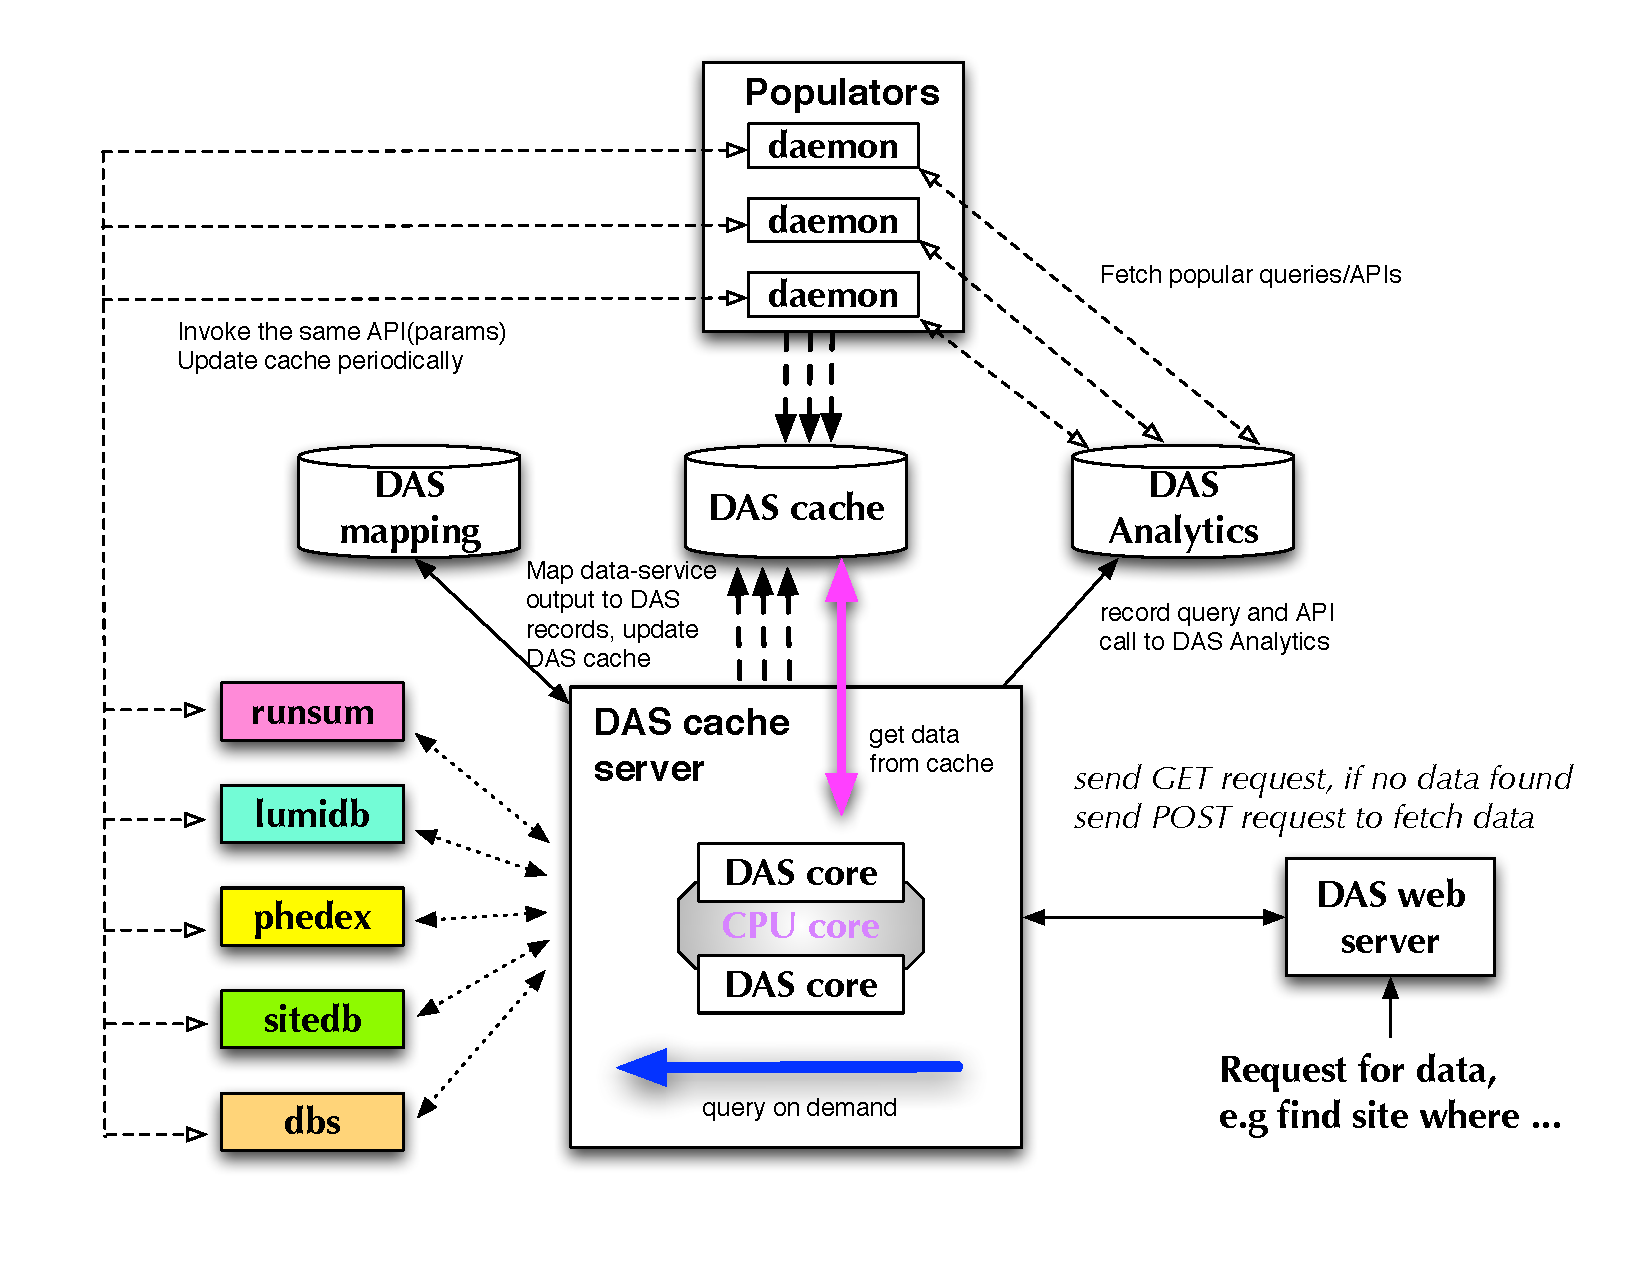
\includegraphics[width=100mm]{DAS_Cache_and_Analytics.pdf}
\caption{
The DAS architecture diagram. 
Input query where placed into analytics DB and mapped into set of
data-service APIs and their parameters. If superset of the query has been
found in DAS cache, the appropriate results were delivered back to users.
Otherwise a data-service APIs were invoked, triggering DAS cache population. 
Once data become available and aggregated in DAS cache users were able 
to see the results. This on demand system was supplemented by DAS robots 
(unix daemons) who were consulting DAS analytics database to enable data 
population into DAS cache for most common query requests.
}
\label{DAS_cache}
\end{figure}

\noindent
Based on this set we rule out the choice of RDMS as DAS back-end(s)
for several reasons. We agreed to support dynamic queries, data
aggregation on demand and pluggable data-services. Therefore a choice 
of concrete schema for data storage was problematic. Moreover we didn't impose
any transactions and data persistency in DAS. This allows us to look 
for alternative IT solutions.
Through the analysis of available options, such as a file-based and memory caches, 
key-value databases, documented-oriented databases we made our choice in favor 
of the last technology. Among them we evaluated CouchDB \cite{CouchDB} and 
MongoDB \cite{MongoDB}. Both systems provide schema free document
storage, replication and fail-over features, but our choice in favor of 
MongoDB was obvious, due to its support of dynamic queries, 
full indexies, including inner objects and embedded arrays,
and auto-sharding. Our prelimiary benchmarks shown that it can sustain
the desired load and size of our meta-data information. We used 
document-oriented database, MongoDB, as a back-end for the three 
main DAS components: Mapping, Analytics and DAS cache databases, 
which will be discussed next. 

The DAS architecture is shown in Fig. \ref{DAS_cache}. It consists of
core library with support of pluggable modules for data retrieval;
caching layer to store data-service output and aggregated results;
request service to handle user queries;
Mapping DB to keep information about data-service APIs, their
notations and mapping to DAS;
Analytics DB for query analysis and identification of pre-fetch 
strategies.

\subsection{DAS core}
The DAS core communicates with different data-services and retrieves
data on demand. This was done by invoking appropriate data-service plugin
upon the user request. Each plugin consists of DAS map, the
data parser(s) to convert data-service output into DAS records
and it was responsible for data-service API calls.
The data-service DAS map contains information about data-service APIs,
input and output parameters and their mapping to DAS keys. 
This information was stored into DAS Mapping DB which we discuss next.
Below you can see a typical DAS Mapping DB record for CMS
SiteDB data-service \cite{SiteDB}:
%\footnote{We used regular expression 
%patterns, evaluated during run time, to validate provided set of input 
%paremters and DAS keys.}:
\begin{verbatim}
{"api":{"params":{"name":""}, "name":"CMSNametoSE"}, "system":"sitedb",
 "api2das": [{"pattern": "re.compile('^T[0-3]_')", 
              "api_param": "name", "das_key": "site"}], 
 "daskeys": [{"pattern": "re.compile('^T[0-3]_')", 
              "key": "site", "map": "site.name"}]}
\end{verbatim}
Although the majority of data-services looks alike
and their logic was abstracted, including parsers, there were a few
cases where special care was required. For instance,
to deal with data-services which were only accessible via private network.
Therefore, a way to propagate user credentials was required, leading
to specific plugin implementation.

%All user queries were written to Analytics DB for further analysis, while
%mapping between data services were kept in Mapping DB. The data-service 
%output were re-mapped into DAS notations and, if necessary, aggregated 
%inside of the DAS cache.

\subsection{DAS Mapping DB}
DAS Mapping DB holded the mapping between data-service APIs and DAS keys exposed to
the users. It created a necessary glue between data-services and identifies
how their data can be related to each other. Basically Mapping DB was positioned 
as a {\it registration} service with ability to translate notations among data-services.
Upon identification of APIs which will participate in DAS activity 
we stored their names, input parameters, together with their type and accept 
values as regular expression patterns into the Mapping DB. 
Also we stored the mapping between data-service notations and DAS keys. 
For instance, the CMS DBS system \cite{DBS}
used \verb+logical_file_name+ notation to identify the name of the
logical file, while the same entity was called \verb+lfn+ 
in CMS PhEDEx system \cite{PhEDEx}.
Since both of them were referred to the logical file name, 
we map both notations into DAS key \verb+file+.
%\footnote{We
%also deal with physical file names, but still used {\it file} to refer to them in
%DAS notations, since simple regular expressions were used to identify the
%meaning of the {\it file} keyword from the provided value.}
Such keys, e.g. \verb+file+, were exposed to the end-users as pre-defined keywords to
be used in search queries. For instance, end-users were able to type \verb+file+ in
order to get all file names known to DAS via data-services as well as
provide a concrete patterns associated with a file, e.g. \verb+file = abc*+.
Under the hood, the appropriate data-service APIs were looked up along with appropriate
parameters to answer those questions. In aforementioned example, 
usage of \verb+file+ in DAS query cause a call of DBS 
\verb+listFiles+ and PhEDEx \verb+fileReplicas+ APIs, respectively.
This approach gave power to end-users to express the meaning of their queries, especially
when they deal with numbers, and achieve accuracy of results. 
For instance, users were able to type \verb+run > 10 and run < 100+
to specify a range of run numbers to be looked up in DAS cache. At the same time
a full keyword search is under development.
% within MongoDB.

\subsection{DAS Analytics DB}
The DAS Analytics DB played a special role. It collected information
about user requests placed to the system. Each request was recorded. Upon its
decomposition into set of selection keys and conditions we also recorded
API name and input parameters into the Analytics database and 
keep updating their counter information for repeated calls. 
This allows to keep track of frequency of API calls and establish 
pre-fetch strategies for most common queries.

\subsection{DAS caching system}
The DAS caching system was used to dynamically fetch
and aggregate data upon user requests. We used the following 
algorithm:
\begin{enumerate}[1.]
\item Decompose query into set of conditions ($conds$) 
and selection keys ($skeys$)
\item Check cache for query hash, if found: look-up results from the cache
\item Identify list of APIs which can serve requested data
\begin{verbatim}
apilist = [r(url, api, args) for r in mapping_db(skeys, conds)]
\end{verbatim}
Here \verb+mappind_db+ defines translation between input query and data-service
APIs which can delivery such data.
\item Iterate over APIs
\begin{verbatim}
for url, api, args in apilist:
    if  superset_in_analytics(api, args):
        continue
    for row in parser(get_data(url, api, args)):
        yield row
\end{verbatim}
Here \verb+superset_in_analytics+ identifies if provided \verb+api, args+
are subset of already registered in Analytics DB api call(s). The 
\verb+get_data+ and \verb+parser+ are define methods to fetch and parse
data, respectively.
\item Perform aggregation by iterating over records from the previos step
\begin{verbatim}
if cache_has(row.primary_key):
   existing_record = get_from_cache(row.primary_key)
   merge(row, existing_record)
   insert_into_cache(row)
   delete_from_cache(existing_record)
else:
   insert_into_cache(row)
\end{verbatim}
We did use a bulk insert operations to increase throughput. The \verb+primary_key+
is a key which identify the record defined in Mapping DB, e.g. \verb+file.name+
for \verb+file+ record.
\item Get results from the cache
\end{enumerate}
%The data was stored in a form of DAS records into the cache, while
%queries were recorded into Analytics DB for further analysis.
We also had an option to run independent set of daemons, DAS robots, who
monitor Analytics DB for most popular requests and pre-fetch the most
common data into DAS cache. 
%The interesting part was being able
%to identify the superset of api/args out of found one in an Analytics DB.

%The DAS caching system was used to store data-service results and aggregated
%information in form of DAS records. As it shown in figure \ref{DAS_cache} 
%the DAS cache server updates Analytics DB, requests and retrieve data from DAS cache
%and aggregate data over there. The independent set of daemons, DAS robots, were
%constantly monitor Analytics DB for most popular requests and pre-fetch most
%common data into DAS cache.

%Each user request placed to the system was parsed and set of selection
%and condition keys were identified. They were mapped into set of
%data service APIs and their input parameters. DAS
%cache was checked for a queries with a similar set of selection and condition
%keys used earlier.\footnote{Since DAS didn't hold
%any data by default we cannot rely on data being present in a cache.
%Moreover if we look-up data first, we cannot tell if it was complete
%set or not, since earlier queries may retrieve only portion of the requested data.}
%If the superset was found a data were
%retrieved from the cache, otherwise a data-service APIs were
%invoked and the results were collected and aggregated inside of DAS cache.

\subsection{DAS queries}
Apart from previous DBS-QL syntax we decided to drop its syntax and allow users
express their queries in a free text-based form. Although we must clarify its
meaning. We used a pre-defined set of keys registered in DAS to describe common
entities of our data. For example, \verb+dataset+, 
\verb+file+, \verb+block+, \verb+run+, \verb+event+. Those
names were used by our users in their daily work operations. So, by typing a
\verb+file+ we didn't perform a string matching to the 
``file'' string, but rather look-up all file objects in a DAS. 
Moreover each DAS key has a default attribute.
For intance, the default attribute for
\verb+dataset+, \verb+block+, \verb+file+ 
was a \verb+name+, while the default attribute for
\verb+run+ and \verb+event+ was a \verb+number+. 
This allows to specify key-value pair as simple as possible, e.g.
\verb+run=123456+, which means run number 123456. At the same time a query 
key, e.g. \verb+site+ meant to look-up all site objects. Such ability
to use key-value pairs resolve ambiguity in object values. For instance,
specifying a run number as \verb+run=123456+ instructs system to resolve
data object with run equal to 123456 rather then other objects which may have
123456 values, e.g. event number or file size. At the same time, to complement
the stregth of the DAS we do plan to index data objects and add a keyword-based 
search later.

The free text-based queries were transformed into MongoDB query syntax, 
who was used internally in DAS. It represents a set of selection 
keys and conditions as a JSON document. For example, a query
{\it dataset site=T1\_CH\_CERN}
was transformed into 
{\it \{"fields" : ["dataset"], "spec" : \{"site" : "T1\_CH\_CERN"\}\}}.
Such syntax was perfect fit for us, since it allows to store all queries
as JSON documents into Analytics DB for further analysis. It is worthwhile to note that
MongoDB query syntax is very reach. It supports advanced queries with 
boolean expressions, conditional operators, regular expressions, etc. providing
a real power for our end-users.

\subsection{Data-services and aggregation}
As we outlined above the DAS Mapping DB becomes an authorative
source of information about all data-services participating in DAS.
Based on information stored in Mapping DB we were able to 
retrieve appropriate data from different data-services, re-map them into 
DAS notations and aggregate them on demand. For instance, the Data 
Bookkeeping System (DBS) and data location system (PhEDEx)
provided information about CMS data block objects. In former case, DBS 
stored information about blocks and their relationships to other 
physics objects, such as dataset adn files, while PhEDEx kept
information about its location and replicas. Upon a user request to 
find a block, we were able to identify appropriate set of DBS and PhEDEx APIs, 
retrieve data from them, re-format their output to DAS notations 
and store results into DAS cache performing aggregation of matched 
objects using \verb+block.name+ key. The merged results were stored 
as a set of data records. Here is an example of such aggregated record:
\begin{verbatim}
{"das_id": ["4b195404e2194e21c4000030", "4b1953fee2194e21c4000002"], 
 "block": [{"name": "/a/b/c#123", "replica": [{"complete": "y", 
            "subscribed": "n", "custodial": "n", "site": "T1_US_Buffer", 
            "nfiles": "18", "se": "srm.site.com", 
            "size": "112694171838"}, {....}]},
           {"name": "a/b/c#123", "nevents": "570200", 
            "created_by": "USER_DN", "path": "/a/b/c", ...}],
 "das": [{"expire": 1259952908}, {"expire": 1259954702}]}
\end{verbatim}
Here \verb+das_id+ refers to api call records stored in Analytics DB,
\verb+block+ represents an aggregation block object information from DBS
and PhEDEx systems and \verb+das+ contains their expiration time stamps.
Usage of this information was valuable contribution in debugging process of
data-services themselves, e.g. identification of not-matched records, 
latency studies, etc.
% Here is an example of DAS record representing
%aggregation information between two SiteDB APIs, {\it CMStoSAMName} 
%and {\it CMStoSiteName}, with API results merged under the {\it site} key.
%\begin{verbatim}
%{"site":[{"samname": "CERN-PROD", "name": "T1_CH_CERN"}, 
%         {"sitename": "CERN", "name": "T1_CH_CERN"}], 
% "das": [{"ctime": 0.9, "expire": 1256362175, "api": ["CMStoSAMName"],
%          "url": "https://a.b.com/sitedb/json/index/CMStoSAMName", 
%          "timestamp": 1256318975, "system": ["sitedb"]},
%         {"ctime": 1.2, "api": ["CMStoSiteName"], "expire": 1256362174},
%          "url": "https://a.b.com/sitedb/json/index/CMStoSiteName", 
%          "timestamp": 1256318974, "system": ["sitedb"]]}
%\end{verbatim}

%We used RESTful model \cite{REST} for all DAS cache server APIs.
%It allows us to share core library and other components during development of 
%various DAS clients, e.g. CLI, web interface, robots, etc. and hides
%complexity of access to individual data-services and their security policies
%as well as proper organize caching solution.
%For instance, to access on-line Run Summary information we were forced to use
%Grid certificates. Instead of propagating user certificate to data-service
%the DAS cache server works as a proxy to this server and used host certficiate 
%to serve such requests on behalf of the users.

\section{Results\label{Results}}
In this section we discuss preliminary restults achieved with DAS system
using the following CMS data-services:
\begin{itemize}
\item Data Bookkeeping System, DBS \cite{DBS}, the CMS meta-data service;
\item Physics Experiment Data Export, PhEDEx \cite {PhEDEx}, the 
CMS file transfer system;
\item SiteDB \cite{SiteDB}, the CMS site resources data-service;
\item RunSummary \cite{RunSummary}, the CMS run and trigger data-service;
%\item LumiDB \cite{LumiDB} collects information about Luminosity conditions;
%\item DQ \cite{DQ}, Data Quality data-service which collects information
%about detector conditions during data taking;
%\item Overview \cite{Overview}, collects information about CMS
%transfer rate, etc.;
\item Dashboard \cite{Dashboard}, the LHC virtual organization
monitoring data-service portal;
\end{itemize}
Each data-service has its own scope, size and peculiar properties. 
For instance, the data in PhEDEx are transient due to constant 
migration of CMS data; the DBS system were divided into dozen 
of individual instances with own size and lifetime, who has been used by different production 
teams for various bookkeeping tasks; the RunSummary data-service
operates on private network accessible at CMS online operation center.
%Table \ref{db_size} shows the current size of meta-data from aforementioned 
%data-services.
%\begin{figure}[htb]
%\centering
%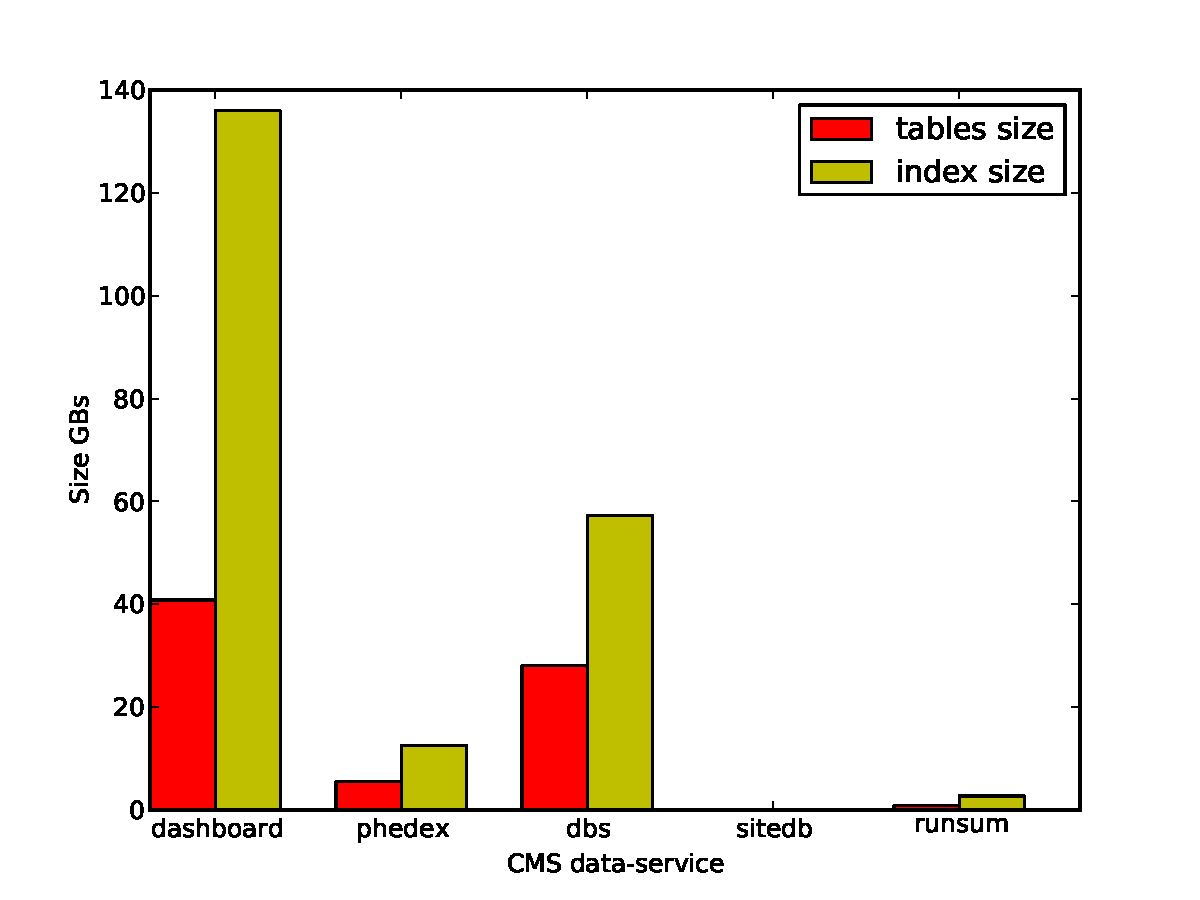
\includegraphics[width=100mm]{db_size.pdf}
%\caption{
%Current size of meta-data for CMS data-services participated in DAS, before
%official data-taking. 
%}
%\label{db_size}
%\end{figure}

%\begin{table*}[hbt]
%\centering
%\begin{tabular}{llllll}\hline
%\hline

%Size of  & Dashboard & DBS & PhEDEx & SiteDB & RunSummary \\
%\hline
%tables (GB) & 40.8  & 28.0 & 5.5 & 0.006 & 0.9 \\
%indexies (GB) & 135.9 & 57.2 & 12.6 & 0.004 & 2.7 \\
%\hline
%\hline
%\end{tabular}
%\caption{
%Current size of meta-data for CMS data-services participated in DAS, before
%official data-taking. 
%}
%\label{db_size}
%\end{table*}
At the moment their size is quite small ranging from 1 to 40 GB and 2 to 140 GB in
table and index sizes, respectively. But we estimate to accumulate $\sim$500 GB of 
meta-data each year during normal CMS operation at LHC.
%\footnote{This number is based on tests 
%performed in CMS during Cosmic Run at Full Tesla (CRAFT) data taking \cite{CRAFT09}.}
%In CRAFT09 acquisition era, Tier-0 produced a total of 6.03
%billion events, 330TB in 32 datasets:
%AlCa/Calibration RAW: 926 million events, 29TB
%Physics RAW: 1.24 billion events, 147TB
%PromptReco: 1.24 billion events, 111TB
%Bulk ALCARECO: 2.34 billion events, 11TB
%Express FEVT: 105 million events, 24TB
%Express ALCARECO: 153 million events, 0.99TB
%HLTMON FEVTHLTALL: 31 million events, 7.4TB
%Above event numbers have signicant overlap by design, 
%2.2 billion unique events, including 524 million cosmic muon
%triggers
% 0.3PB - 50GB meta-data in DBS
% 3PB/y - x GB

To test DAS performance we measured elapsed time and CPU/RAM utilization
required to collect and aggregate information from different
data-services. Table \ref{DAS_benchmark} summarizes the biggest 
contributors so far, the block information between DBS and 
PhEDEx CMS data-services. 

\begin{table*}[hbt]
\centering
\begin{tabular}{llllll}\hline
\hline
System & Format & Size & Records & Elapsed time & Elapsed time \\
& & & & no cached data & w/ cached data \\
\hline
DAS (DBS) & XML & 187MB & 368716 & 53 sec & 0.92 sec \\
DAS (PhEDEx) & XML & 164MB & 175884/170131 & 160 sec & 0.94 sec \\
DAS (aggregate) & JSON & 357MB & 374468 & 256 sec & 44.8 sec \\
\hline
\hline
\end{tabular}
\caption{Time required to fetch, parse and aggregate block information
from DBS and PhEDEx systems. In the case of PhEDEx
system we show total number of fetched records 175884 together with
number of records merged in DAS 170131. The total number of DAS records 
were calculated as number of aggregated records plus left overs,
the non-matched records from both systems.}
\label{DAS_benchmark}
\end{table*}

Please note that initial DAS implementation was done in Python 
and all tests were performed on x64 Linux platform with 16GB of RAM where
1 CPU was used by DAS server and 1 CPU by MongoDB database server. The CPU utilization
of DAS server was 67\% in average and RAM usage was below 35MB. 
All tests were performed multiple times to avoid fluctuations. 
The elapsed time measured during those tests consists of the 
following componenets:
\begin{itemize}
\item[]
{\it
Elapsed time = retrieval time + parsing time + re-mapping time 
        + cache insertion/indexing time 
        + (aggregation time) + (output creation time)
}
\end{itemize}
Here the {\it retrieval time} is a time required to access data from remote data-service,
{\it parsing time} is a time required to read and parse received data, {\it re-mapping time}
is a time required to convert notations used by data-service to DAS ones for every object
we parse, {\it cache insertion} and {\it indexing time} represents time spend to add objects into
the DAS cache, {\it aggregation time} is required to merge objects into DAS records based
on their common key (block name in this case) and {\it output creation time}
is a time required to write DAS records to disk. Please note that last two
components, {\it aggregation} and {\it output creation time}, were only applied to
the one of the sub-system (either DBS or PhEDEx) since the first one was injected into
the fresh database, while the second required the merging step.

%DAS execution time (phedex) 160.606897116 sec
%DAS execution time (dbs) 52.5349619389 sec
%DAS execution time 256.0670228 sec, Sat, 28 Nov 2009 15:46:39 GMT
%
%DAS execution time (phedex) 0.952513933182 sec
%DAS execution time (dbs) 0.951184034348 sec
%DAS execution time 44.7982931137 sec, Sat, 28 Nov 2009 15:52:11 GMT

The individual tests of DAS components (DBS and PhEDEx) shown roughly 
the same performance. Although the time of PhEDEx component was bigger 
due to longer retrieval and parsing time.
The time of PhEDEx component shown in Table \ref{DAS_benchmark} divided 
among: retrieval + parsing step, $\sim$110 sec, and merging step, $\sim$50 sec.
As shown in Table \ref{DAS_benchmark},
the time spent to access individual components (last column) was quite
reasonable, roughly 1 second for both systems. While final time to
get DAS records on disk was about 45 seconds. This was mostly due to I/O and
conversion operations between binary data format used by MongoDB, BSON, to DAS
data format, JSON.

Based on results of stress tests we measured that we can achieve 7000 docs/sec rate
for insertion, 3400 docs/sec for aggregation and 8500 docs/sec for reading operation
in DAS, which is suitable for our needs. Since all operations were performed 
on a single CPU a further improvements are expected. Also, a necessary
tuning can be done by using C++ driver instead of python one.

\section{Summary}
We presented a new data aggregation service (DAS) developed for CMS High-Energy experiment
at LHC, CERN, Geneva, Switzerland. It was designed to provide caching and
aggregation layer on top of the existing relational and non-relation data-services
mostly in real time fashion. All of the data were retrieved on demand basis,
while data pre-fetching of most common queries is in our plans. We developed
prototype in python for DAS system which is under commissioning phase right now 
and presented performance studies in this paper. 
The CMS experiment is started to collect its data in December of 2009 and 
we expect to accumulate a few PB of real data each year to tape. 
In addition, the Monte-Carlo samples will be produced at this scale.
Based on test studies performed in CMS, we expect that total size of
meta-data produced by experiment each year will be of the order of
500GB. The DAS should sustain such load and will provide generic 
``data-discovery'' service for CMS experiment in years to come.

\section{Acknowledgments}

This work was supported by the National Science Foundation and 
Department of Energy of the United States of America. 
Fermilab is operated by Fermi Research Alliance, LLC under Contract
No. DE-AC02-07CH11359 with the United States Department of Energy.

%% References
%%
%% Following citation commands can be used in the body text:
%% Usage of \cite is as follows:
%%   \cite{key}         ==>>  [#]
%%   \cite[chap. 2]{key} ==>> [#, chap. 2]
%%

%% References with BibTeX database:

%\bibliographystyle{elsarticle-num}
%\bibliography{<your-bib-database>}

%% Authors are advised to use a BibTeX database file for their reference list.
%% The provided style file elsarticle-num.bst formats references in the required Procedia style

%% For references without a BibTeX database:

% \begin{thebibliography}{00}

%% \bibitem must have the following form:
%%   \bibitem{key}...
%%

% \bibitem{}

% \end{thebibliography}

\section*{References}
\begin{thebibliography}{00}
\bibitem{DBXplorer}
S. Agrawal, S. Chaudhuri, G. Das,
``DBXplorer: A System for Keyword-Based Search over Relational Databases'',
ICDE 2002, pp. 5-16.

\bibitem{QueryAnswer}
G. Koutrika, A. Simitsis, Y. E. Ioannidis,
``Pr\'{e}cis: The Essence of a Query Answer'',
ICDE 2006, pp. 69-78.

\bibitem{DBS-QL} 
V. Kuznetsov, D. Riley, A. Afaq, V. Sekhri, Y. Guo, L. Lueking,
``The CMS DBS Query Language'', CHEP 2009.

%\bibitem{AMI}
%Altas AMI web portal,
%http://ami.in2p3.fr/opencms/opencms/AMI/www/Tutorial/AMIMediation.html

\bibitem{FedDB}
L. Haas, E. Lin,
``IBM Federated Database Technology'', \\
http://www.ibm.com/developerworks/data/library/techarticle/0203haas/0203haas.html

\bibitem{CMS} 
R. Adolphi et al., 
``The CMS experiment at the CERN LHC'',
JINST 0803, S08004 (2008).

\bibitem{CMSDataModel} 
C. Grandi, D.Stickland, L.Taylor et al.,
``The CMS Computing Model'',
CERN-LHCC-2004-035/G-083 (2004).
%A. Fanfani et. al., 
%``Distributed Analysis in CMS'', 
%to be published in Journal of Grid Computing.

\bibitem{iRODS}
The Integrated Rule-Oriented Data System,
http://www.irods.org/

\bibitem{OpenArchive}
Open Archives Initiative,
http://www.openarchives.org/

\bibitem{DBS} 
A. Afaq, et. al.,
``The CMS Dataset Bookkeeping Service'', 
J. Phys. Conf. Ser, 119, 072001 (2008).

\bibitem{DBS07} 
A. Dolgert, V. Kuznetsov, C. Jones, D. Riley, 
``A multi-dimensional view on information retrieval of CMS data'',
J. Phys. Conf. Ser, 119, 072013 (2008).

\bibitem{DD} https://cmsweb.cern.ch/dbs\_discovery

\bibitem{Arms}
C. R. Arms, W. Y. Arms,
 ``Mixed Content and Mixed Metadata 
Information Discovery in a Messy World'',
chapter from ``Metadata in Practice'', ALA Editions, 2004.

\bibitem{MySQL}
http://www.mysql.com/

\bibitem{CouchDB}
http://couchdb.apache.org/

\bibitem{MongoDB}
http://www.mongodb.org/

%\bibitem{REST}
%Fielding, Roy Thomas ``Architectural Styles and the Design of 
%Network-based Software Architectures'', Doctoral dissertation, 2000,
%University of California, Irvine

\bibitem{PhEDEx}
%Rehn et. al.,
%``PhEDEx high-throughput data transfer management system'', CHEP 2006;
%R. Egeland et al., 
%``Data transfer infrastructure for CMS data taking'', 
%Proceedings of Science, PoS (ACAT08) 033 (2008);
L. Tuura et al., 
``Scaling CMS data transfer system for LHC start-up'', 
J. Phys. Conf. Ser, 119, 072030 (2008).

\bibitem{RunSummary}
https://cmswbm.web.cern.ch/cmswbm/cmsdb/servlet/RunSummary

\bibitem{SiteDB}
https://cmsweb.cern.ch/sitedb/

%\bibitem{LumiDB}
%https://twiki.cern.ch/twiki/bin/view/CMS/CMS-DMWM-DBS-Luminosity

%\bibitem{DQ}
%Data-Quality DB reference

%\bibitem{Overview}
%https://cmsweb.cern.ch/overview/

\bibitem{Dashboard}
J. Andreeva, et. al,
``Experiment Dashboard – The Monitoring System for the LHC Experiments'',
GMW’07, June 25, 2007, Monterey, California, USA.

%\bibitem{CRAFT09}
%https://twiki.cern.ch/twiki/bin/view/CMS/CRAFT09AnalysisInfo

%\bibitem{Python} Python programming language, http://www.python.org

%\bibitem{DBSearch}
%D. Konopnicki, O. Shmueli,
%``Database-Inspired Search'', 
%Proc. of the 31st VLDB Conference, 2005.
\end{thebibliography}
\end{document}
